\documentclass{standalone}

\usepackage{tikz}
    \usetikzlibrary{arrows.meta}
    \usetikzlibrary{calc}
    \usetikzlibrary{decorations.pathmorphing}

\tikzset{
    bluearrow/.style={
        blue!25,
        -{Kite[length=2.5mm]}, 
        line width=0.5mm,},
    greensq/.style={
        green,
        fill=green!20, 
        line width=0.4mm,},
    redsq/.style={
        red,
        fill=red!20, 
        line width=0.4mm,},
    }
    
\begin{document}
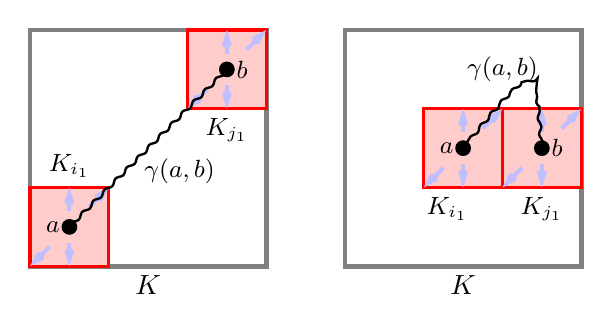
\begin{tikzpicture}
    % \draw[help lines] (0,0) grid (15,3);
    \foreach \x in
        {(0,0), (4,0)} 
        {\draw[black!50, line width=0.6mm] \x rectangle+(3,3);}
    \foreach \x in
        {(0,0), (2,2), (5,1), (6,1)} 
        {\draw[redsq] \x rectangle+(1,1);}
    \fill[black] 
        (0.5,0.5) circle (1mm)
        (2.5,2.5) circle (1mm)
        (5.5,1.5) circle (1mm)
        (6.5,1.5) circle (1mm);
    \foreach \x in
        {(0,0), (2,2), (5,1), (6,1)} 
        {\draw[bluearrow] \x++(0.25,0.25) -- ++(-0.25,-0.25);
         \draw[bluearrow] \x++(0.75,0.75) -- ++(.25,0.25);
         \draw[bluearrow] \x++(0.5,0.3) -- ++(0,-0.3);
         \draw[bluearrow] \x++(0.5,0.7) -- ++(0,0.3);}
    \draw[line width=0.3mm, decorate, decoration={coil,aspect=0,segment length=2mm,amplitude=0.2mm}]
        (0.5,0.5)--(2.4,2.4) 
        (5.5,1.5)..controls(6.4,2.6)..(6.5,1.5);
    \node[shift={(1.9,1.2)}]{\small$\gamma(a,b)$};
    \node[shift={(1.5,0)}, below]{$K$};
    \node[shift={(0.5,1)},above]{\small$K_{i_1}$};
    \node[shift={(2.5,2)}, below]{\small$K_{j_1}$};
    \node[shift={(0.5,0.5)},left]{\small$a$};
    \node[shift={(2.5,2.5)}, right]{\small$b$};
    
    \node[shift={(6,2.5)}]{\small$\gamma(a,b)$};
    \node[shift={(5.5,0)}, below]{$K$};
    \node[shift={(5.3,1)},below]{\small$K_{i_1}$};
    \node[shift={(6.5,1)}, below]{\small$K_{j_1}$};
    \node[shift={(5.5,1.5)},left]{\small$a$};
    \node[shift={(6.5,1.5)}, right]{\small$b$};
\end{tikzpicture}
\end{document}